\documentclass[a4paper]{report}
\usepackage[brazil]{babel}
\usepackage{graphicx}

\begin{document}
\section{por tr\'as das cortinas}
Essa \'e uma hist\'oria que foi vivenciada e escrita por um motorista mas narrada por um autom\'ovel 
fabricado no brasil, desenhado por uma garota, filha de um empresario carioca que admninistrava  uma f\'abrica de
 implementos agricolas e ferroviarios no munic\'ipio de entre rios.

Devido aos diversos acontecimentos, que ao longo do tempo vivenciei, tive a ideia de 
registrar as coisas mais interessantes pois sei que daqui pra frente vai ser cada vez mais dif\'icil algu\'em vicenciar,
tais acontecimentos, tanto pela modernidade e complexidade gradual dos meios de transporte dispon\'iveis, quanto pela propria
natureza humana de querer sempre facilitar e tornar mais confortavel a vida se afastando cada vez mais da aventura e do instinto.

Pra mim \'e isso que significa um autom\'ovel antigo, afastar um passo do materialismo, da moda, da preocupa\c{c}\~ao natural de nossos dias
e aproximar um passo do natural, do divertido, do instinto e de tudo que da gra\c{c}a a vida, a aventura, a emo\c{c}\~ao.

\'E disso que se trata esse livro, o prazer da vida contado por uma maquina de 6 cilindros, 4 rodas e um cora\c{c}\~ao.

Agrade\c{c}o a todos os amigos(as) que fizeram parte desta aventura, e desde j\'a dedico esta obra a todos vo\c{c}\^es.

\section{Pref\'acio: O in\'icio de um sonho}
Nos anos 80, quando eu tinha meus 11 anos, havia uma santa matilde branco perolada na minha cidade,
eu passava por ela algumas vezes, indo ou voltando da escola, sempre achei o carro mais bacana de todos.

\begin{figure}[!htb]
\centering
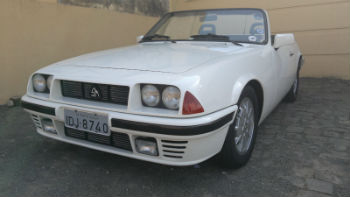
\includegraphics{sm_bco_per}
\caption{SM branco Perolado}
\label{sm_bco}
\end{figure}

Certo dia, pela manh\~a, seu Louren\c{c}o, meu falecido pai, me pediu para ligar o carro para aquecer o motor,
mesmo n\~ao sendo necess\'ario para um carro relativamente moderno para \'epoca, para mim foi uma experi\^encia \'unica,
at\'e aquele momento, eu nunca havia ligado um carro, pra mim foi um divisor de \'aguas para a vida adulta.

Obviamente eu n\~ao fazia ideia do funcionamento da embreagem e da marcha, liguei o carro com a marcha engatada e por sorte
nao demoli a frente do carro, foi a unica e ultima vez que tive a chance de fazer aquilo, mas a emo\c{c}\~ao do motor ligando ficou
na minha mem\'oria, naquele mesmo ano vi mais algumas vezes a SM branco perolado e pensei que se algum dia eu pudesse ter um
autom\'ovel, seria uma SM, esse dia chegou em 2011.

Eu estava visitando uns amigos em rio grande e fui convidado para almo\c{c}ar \`a bordo com a tripula\c{c}\~ao do Atl\~antico Sul, o navio
oceanog\'afico da FURG.

Durante o almo\c{c}o o assunto se dirigiu para autom\'oveis, lembrei do meu antigo sonho e compartilhei com o pessoal, nesta ocasi\~ao um dos marinheiros
me falou que havia uma santa matilde a venda em tapes, um conhecido.

Meu amigo Stefan, que havia me convidado para o almo\c{c}o com sua equipe de trabalho, entusiamou-se com a informa\c{c}\~ao, e obviamente eu tambem, e na semana 
seguinte fomos com mais um amigo de rio grande, Daniel Torres, vulgo "bala", outro entusiasta dos 6cilindros, ver a preciosidade.

Durante o trajeto, rio grande - tapes, conversamos muito,   


























\end{document}
